\documentclass[12pt, psamsfonts]{amsart}

%-------Packages---------
\usepackage{amssymb,amsfonts}
\usepackage{fullpage}
\usepackage[all,arc]{xy}
\usepackage{enumerate}
\usepackage{physics}
\usepackage{mathrsfs}
\usepackage{theoremref}
\usepackage{graphicx}
\usepackage[bookmarks]{hyperref}

%--------Theorem Environments--------
%theoremstyle{plain} --- default
\newtheorem{thm}{Theorem}[section]
\newtheorem{cor}[thm]{Corollary}
\newtheorem{prop}[thm]{Proposition}
\newtheorem{lem}[thm]{Lemma}
\newtheorem{conj}[thm]{Conjecture}
\newtheorem{quest}[thm]{Question}

\theoremstyle{definition}
\newtheorem{defn}[thm]{Definition}
\newtheorem{defns}[thm]{Definitions}
\newtheorem{con}[thm]{Construction}
\newtheorem{exmp}[thm]{Example}
\newtheorem{exmps}[thm]{Examples}
\newtheorem{notn}[thm]{Notation}
\newtheorem{notns}[thm]{Notations}
\newtheorem{addm}[thm]{Addendum}
\newtheorem*{exer}{Exercise}

\theoremstyle{remark}
\newtheorem{rem}[thm]{Remark}
\newtheorem{rems}[thm]{Remarks}
\newtheorem{warn}[thm]{Warning}
\newtheorem{sch}[thm]{Scholium}

\DeclareMathOperator{\Hom}{Hom}
\DeclareMathOperator{\Id}{Id}

\makeatletter
\let\c@equation\c@thm
\makeatother
\numberwithin{equation}{section}

\bibliographystyle{plain}

\begin{document}

\title{Math 601 Homework (Due 9/11)}
\author{Hidenori Shinohara}
\maketitle

\begin{exer}{(1)}
  Show that $2 \times 2$ matrices give a functor, $M_2$, from the category of rings to itself, $R \mapsto M_2(R)$.
\end{exer}

\begin{proof}
  Let $R, R'$ be rings and $\phi \in \Hom(R, R')$.
  Let $M_2(\phi): M_2(R) \rightarrow M_2(R')$ be defined such that

  \begin{align*}
    (M_2(\phi))\begin{pmatrix}\begin{bmatrix} a & b \\ c & d \end{bmatrix} \end{pmatrix} = 
    \begin{bmatrix} \phi(a) & \phi(b) \\ \phi(c) & \phi(d) \end{bmatrix}.
  \end{align*}

  We claim that $M_2$ is indeed a functor.

 \begin{itemize}
   \item
     Claim 1: For any $\phi \in \Hom(R, R')$, $M_2(\phi) \in \Hom(M_2(R), M_2(R'))$.
     In other words, we want to show that $M_2(\phi)$ is a ring homomorphism for any $\phi$.
     \begin{align*}
       (M_2(\phi))\begin{pmatrix}\begin{bmatrix} a & b \\ c & d \end{bmatrix} + \begin{bmatrix} e & f \\ g & h \end{bmatrix} \end{pmatrix} 
         &= (M_2(\phi))\begin{pmatrix}\begin{bmatrix} a + e & b + f \\ c + g & d + h \end{bmatrix} \end{pmatrix} \\
         &= \begin{bmatrix} \phi(a + e) & \phi(b + f) \\ \phi(c + g) & \phi(d + h) \end{bmatrix} \\
         &= \begin{bmatrix} \phi(a) + \phi(e) & \phi(b) + \phi(f) \\ \phi(c) + \phi(g) & \phi(d) + \phi(h) \end{bmatrix} \\
         &= \begin{bmatrix} \phi(a) & \phi(b) \\ \phi(c) & \phi(d) \end{bmatrix} + \begin{bmatrix} \phi(e) & \phi(f) \\ \phi(g) & \phi(h) \end{bmatrix} \\
         &= (M_2(\phi))\begin{bmatrix} a & b \\ c & d \end{bmatrix} + (M_2(\phi))\begin{bmatrix} e & f \\ g & h \end{bmatrix} \\
     \end{align*}
     \begin{align*}
       &(M_2(\phi))\begin{pmatrix}\begin{bmatrix} a & b \\ c & d \end{bmatrix} \begin{bmatrix} e & f \\ g & h \end{bmatrix} \end{pmatrix} \\
         &= (M_2(\phi))\begin{pmatrix}\begin{bmatrix} ae + bg & af + bh \\ ce + dg & cf + dh \end{bmatrix} \end{pmatrix} \\
         &= \begin{bmatrix} \phi(ae + bg) & \phi(af + bh) \\ \phi(ce + dg) & \phi(cf + dh) \end{bmatrix} \\
         &= \begin{bmatrix} \phi(a)\phi(e) + \phi(b)\phi(g) & \phi(a)\phi(f) + \phi(b)\phi(h) \\ \phi(c)\phi(e) + \phi(d)\phi(g) & \phi(c)\phi(f) + \phi(d)\phi(h)) \end{bmatrix} \\
         &= \begin{bmatrix} \phi(a) & \phi(b) \\ \phi(c) & \phi(d) \end{bmatrix} \begin{bmatrix} \phi(e) & \phi(f) \\ \phi(g) & \phi(h) \end{bmatrix} \\
         &= (M_2(\phi))\begin{pmatrix}\begin{bmatrix} a & b \\ c & d \end{bmatrix} \end{pmatrix} (M_2(\phi))\begin{pmatrix}\begin{bmatrix} e & f \\ g & h \end{bmatrix} \end{pmatrix}
     \end{align*}
     Therefore, $M_2(\phi)$ is indeed a ring homomorphism.
   \item
     For any ring $R$ and the identity function $\Id_R$, $M_2(\Id_R)$ is the identity map on $M_2(R)$ because it maps each element in a given matrix to itself.
   \item
     Let $f \in \Hom(A, B), g \in \Hom(B, C)$.
     \begin{align*}
       (M_2(f \circ g))\begin{pmatrix}\begin{bmatrix} a & b \\ c & d \end{bmatrix}\end{pmatrix}
        &= \begin{bmatrix} (f \circ g)(a) & (f \circ g)(b) \\ (f \circ g)(c) & (f \circ g)(d) \end{bmatrix} \\
        &= \begin{bmatrix} f(g(a)) & f(g(b)) \\ f(g(c)) & f(g(d)) \end{bmatrix} \\
        &= M_2(f)\begin{pmatrix}\begin{bmatrix} g(a) & g(b) \\ g(c) & g(d) \end{bmatrix}\end{pmatrix}\\
        &= M_2(f)\begin{pmatrix}M_2(g)\begin{pmatrix}\begin{bmatrix} a & b \\ c & d \end{bmatrix}\end{pmatrix}\end{pmatrix} \\
        &= (M_2(f) \circ M_2(g))\begin{pmatrix}\begin{bmatrix} a & b \\ c & d \end{bmatrix}\end{pmatrix}.
     \end{align*}
 \end{itemize}
 Therefore, $M_2$ is indeed a functor.
\end{proof}

\begin{exer}{(Problem 4 from More exercises)}
  \begin{enumerate}
    \item
      If $F$ is a functor from category $C$ to a category $C'$ and $G$ is a functor from a category $C'$ to a category $C''$, under what conditions is a composite functor, $G \circ F: C \rightarrow C''$ defined?
    \item
      For a ring $R$ write $GL_2(R)$ for the set of all invertible $2 \times 2$ matrices with entries in $R$.
      List the exercises above and the sections of the handouts which combine to give a proof that $GL_2$ is a functor from rings to groups.
    \item
      For a commutative ring $R$ let $SL_2(R)$ denote the set of all $2 \times 2$ matrices with entries in $R$ and determinant 1.
      Is $SL_2$ a functor from commutative rings to groups?
    \item
      Let $k$ be a field.
      There is a natural right action of $GL_2(k)$ on $\mathbb{P}^1(k)$.
      Write down how an element of $GL_2(k)$ acts on an element of $\mathbb{P}^1(k)$ using homogeneous coordinates.
  \end{enumerate}
\end{exer}

\begin{proof}
$ $
  \begin{enumerate}
    \item
      A composition of two functors is always a functor.
    \item
      Exercise 1 from More exercises shows that $M_2$ is a functor from the category of rings to itself.
      From ``Units as a functor" in the handout from the first lecture, we know that passing from rings to units is a functor from the category of rings to the category of groups.
      Then by composing $M_2$ with the operation to take units, we get $GL_2$.
      Exercise 4(a) from More exercises shows that a composition of two functors is a functor.
      Thus $GL_2$ is a functor.
    \item
      Yes, it is.
    \item
      \begin{align*}
        (x_0 : x_1) \star \begin{bmatrix} a & b \\ c & d \end{bmatrix} = (ax_0 + cx_1 : bx_0 + dx_1).
      \end{align*}
  \end{enumerate}
\end{proof}

\begin{exer}{(Problem 8 from More exercises)}
  Consider the subgroup, $D_5 = \langle (12345), (14)(23) \rangle \subset S_5$.
  \begin{enumerate}
    \item
      Set $a = (12345)$ and compute $a^{-1}$.
    \item
      Set $b = (14)(23)$ and compute $aba^{-1}$.
    \item
      Show that every element in $D_5$ may be written in the form $a^ib^j$ for some $i, j \in \mathbb{Z}$.
    \item
      Compute $\abs{D_5}$.
    \item
      Draw a regular pentagon with vertices labeled successively 1, 2, 3, 4, 5.
      Show that $D_5$ acts on the pentagon by describing he action in geometric terms.
    \item
      Recall that a group acts on its subgroups by conjugation, $H \subset G, H \mapsto gHg^{-1}$.
      The orbits of this action are called conjugacy classes of subgroups.
      Determine all the conjugacy classes of subgroups of $D_5$.
  \end{enumerate}
\end{exer}

\begin{proof}
  $ $
  \begin{enumerate}
    \item
      $a$ sends 1 to 2, 2 to 3, $\cdots$.
      We want $a^{-1}$ to do the opposite.
      Thus $a^{-1} = (15432)$.
      Since $(12345)(15432) = (15432)(12345) = (1)$, $(15432)$ is indeed $a^{-1}$.
    \item
      $aba^{-1} = (a(1)a(4))(a(2)a(3)) = (25)(34)$.
    \item
      $ba = (14)(23)(12345) = (13)(45)$, and $a^{-1}b = (15432)(14)(23) = (13)(45)$.
      Therefore, $ba = a^{-1}b$.
      We claim that $ba^n = a^{-n}b$ for every $n \in \mathbb{N}$.
      Suppose $ba^n = a^{-n}b$ for some $n \in \mathbb{N}$.
      Then $ba^{n + 1} = (ba^n)a = (a^{-n}b)a = a^{-n}(ba) = a^{-n}a^{-1}b = a^{-n-1}b$.
      By mathematical induction, $ba^n = a^{-n}b$ for every $n \in \mathbb{N}$.

      For any $n \in \mathbb{N}$, $ba^n = a^{-n}b$, so $a^nba^n = b$, and thus $a^nb = ba^{-n}$.
      Therefore, we have $ba^k = a^{-k}b$ for every $k \in \mathbb{Z}$.

      We claim that for any $i, j \in \mathbb{Z}$, $b^ja^i$ can be written in the desired form.
      Since $b^2 = e$, we consider two cases based on the parity of $j$.
      If $j$ is even, then $b^j = e$, so $b^ja^i = a^i$.
      If $j$ is odd, then $b^j = b$, so $b^ja^i = ba^i = a^{-i}b$ as shown above.

      We will prove the general case.
      By the argument above, it suffices to show that every element in $D_5$ can be represented as a word of length $\leq 2$.
      Let $x_1^{i_1} \cdots x_k^{i_k} \in D_5$ be given where $i_1, \cdots, i_k \in \mathbb{Z}$ and each $x_i$ is either $a$ or $b$.
      Since $D_5$ is generated by $a, b$, every element can be represented in this form.
      We will show that every element in $D_5$ can be represented as a word of length $\leq 2$ by using strong induction.
      If $k \leq 2$, then we are done.
      Suppose that we can represent every element in $D_5$ of length $\leq k$ as a word of length $\leq 2$ for some $k \geq 2$.
      Let $x = x_1^{i_1} \cdots x_{k + 1}^{i_{k + 1}} \in D_5$.
      If $x_1 = x_2$, then $x = x_2^{i_1 + i_2}x_3^{i_3} \cdots x_{k + 1}^{i_{k + 1}}$, so by the inductive hypothesis, this can be represented as a word of length $\leq 2$.
      If $x_2 = x_3$, then $x = x_1^{i_1}x_2^{i_2 + i_3}x_4^{i_4} \cdots x_{k + 1}^{i_{k + 1}}$, so by the inductive hypothesis, this can be represented as a word of length $\leq 2$.
      Suppose $x_1 \ne x_2$ and $x_2 \ne x_3$.
      Then there are two cases:
      \begin{itemize}
        \item
          Case 1: $(x_1, x_2, x_3) = (a, b, a)$.
          By the argument above, $b^{i_2}a^{i_3}$ can be represented as $a^ib^j$ for some $i, j \in \mathbb{Z}$.
          Therefore, $a^{i_1}(b^{i_2}a^{i_3}) = a^{i_1}(a^ib^j) = a^{i_1 + i}b^j$, so $x$ can be represented as a word of length $k$.
          By the inductive hypothesis, $x$ can be represented as a word of length $\leq 2$.
        \item
          Case 2: $(x_1, x_2, x_3) = (b, a, b)$.
          By the argument above, $b^{i_1}a^{i_2}$ can be represented as $a^ib^j$ for some $i, j \in \mathbb{Z}$.
          Therefore, $(b^{i_1}a^{i_2})b^{i_3} = (a^ib^j)b^{i_3} = a^ib^{j + i_3}$.
          By the inductive hypothesis, $x$ can be represented as a word of length $\leq 2$.
      \end{itemize}
    \item
      \begin{itemize}
        \item
          $a^1 = a \ne (1)$.
        \item
          $a^2 = (13524) \ne (1)$.
        \item
          $a^3 = (14253) \ne (1)$.
        \item
          $a^4 = (15432) \ne (1)$.
        \item
          $a^5 = (1)$.
      \end{itemize}
      Therefore, the order of $a$ is 5.
      Since $b \ne (1)$ and $b^2 = (1)$, the order of $b$ is 2.
      We claim that there are exactly 10 elements in $D_5$.
      \begin{itemize}
        \item
          Claim 1: $\abs{D_5} \leq 10$.
          Let $x \in D_5$.
          Then there exist $i, j \in \mathbb{Z}$ such that $x = a^ib^j$.
          Since the order of $a$ is 5 and the order of $b$ is 2, we can assume that $0 \leq i \leq 4$ and $0 \leq j \leq 1$.
          Therefore, $D_5 \subset \{ a^ib^j \mid 0 \leq i \leq 4, 0 \leq j \leq 1 \}$.
          Thus there are at most 10 elements in $D_5$.
        \item
          Claim 2: $\abs{D_5} \leq 10$.
          Let $a^ib^j, a^{i'}b^{j'} \in \{ a^ib^j \mid 0 \leq i \leq 4, 0 \leq j \leq 1 \}$.
          Suppose $a^ib^j = a^{i'}b^{j'}$.
          Then $a^{i - i'} = b^{j' - j}$.
          We have calculated all the powers of $a$ above, and none of them is equal to $b$.
          Therefore, $i - i' \equiv 0 \pmod 5$ and $j - j' \equiv 0 \pmod 2$.
          Since $0 \leq i, i' \leq 4, 0 \leq j, j' \leq 1$, $i = i'$ and $j = j'$.
          This implies that the set $\{ a^ib^j \mid 0 \leq i \leq 4, 0 \leq j \leq 1 \}$ contains exactly 10 elements.
          Since the set is a subset of $D_5$, $D_5$ contains at least 10 elements.
      \end{itemize}
      Therefore, $D_5$ contains exactly 10 elements.
    \item
      $a$ corresponds to a reflection, and $b$ corresponds to a rotation as in the figure.
       \begin{figure}
         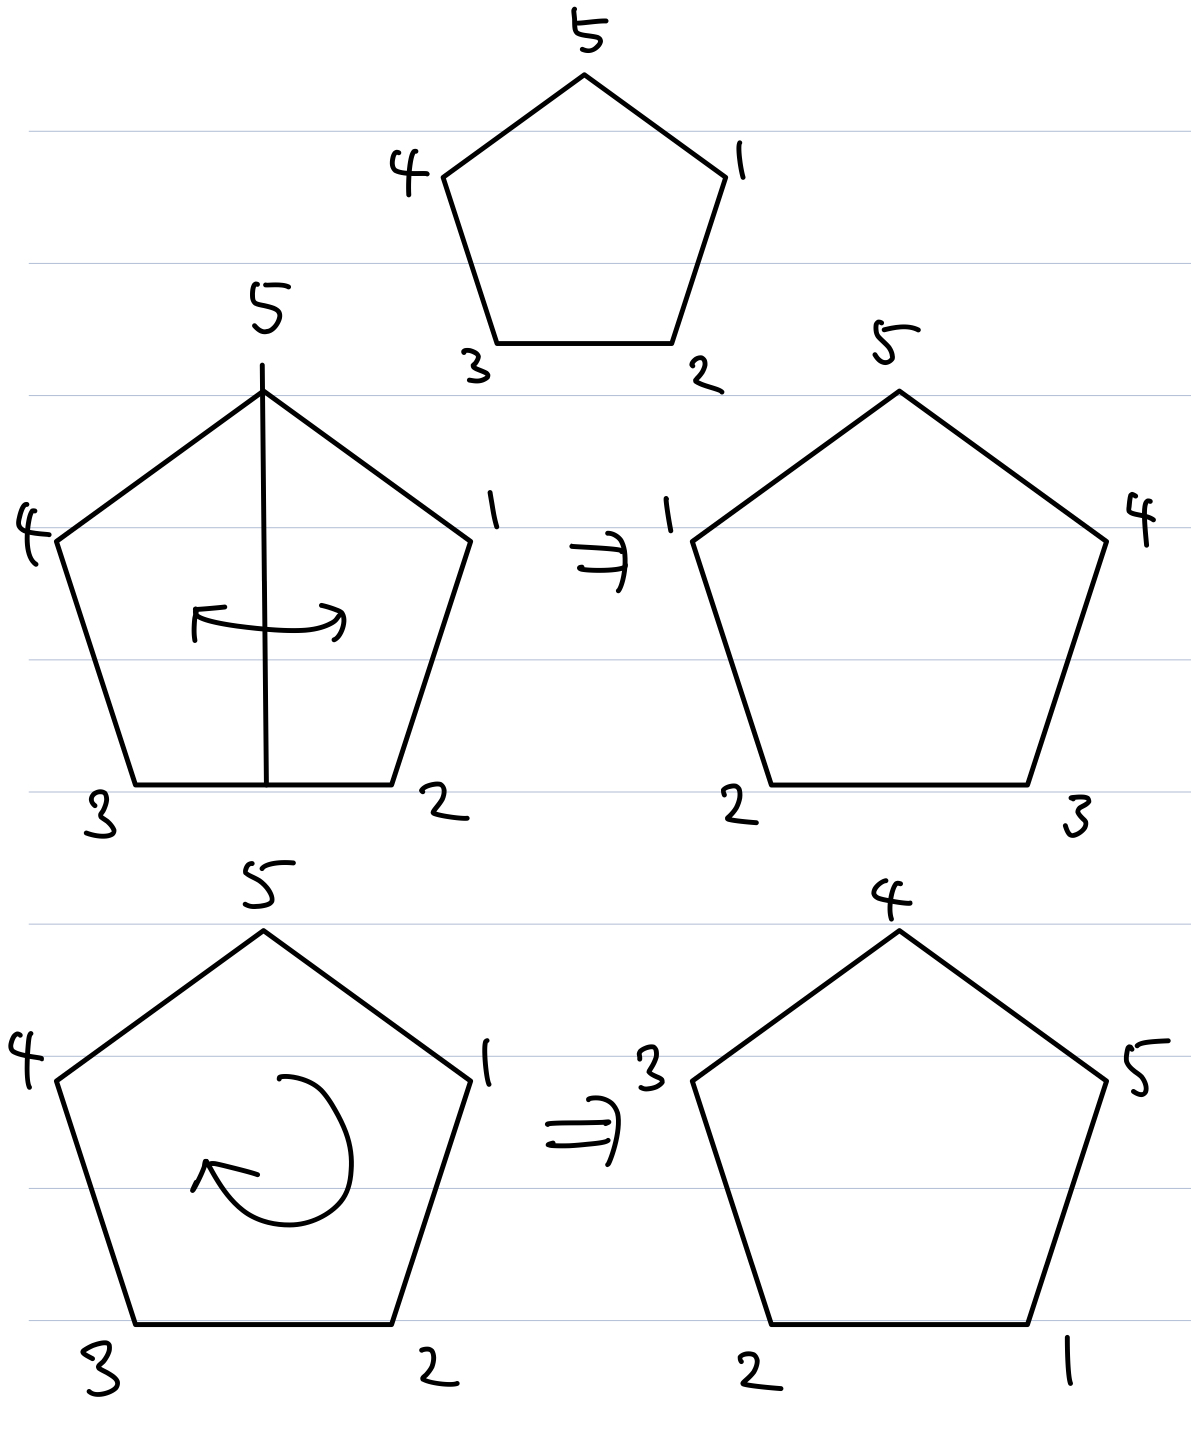
\includegraphics[width=\linewidth]{pentagon.jpg}
           \caption{Interpretate $D_5$ geometrically}
         \label{fig:maps}
       \end{figure}
    \item
       We will first identify all the subgroups of $D_5$.
       By Lagrange's Theorem, a subgroup must have exactly 1, 2, 5, or 10 elements.
       Since the case when the order is 1 or 10 is trivial, we will consider order 2 and 5.
       \begin{itemize}
         \item
           Subgroups of order 2.
           They are cyclic groups generated by elements of order 2.

           $a$ has order 5, so $a$ does not form a subgroup of order 2.
           The order of $a^2, a^3, a^4$ must divide $a^5$ by Lagrange's theorem since $\langle a^i \rangle$ is a subset of $\langle a \rangle$.
           Since $5$ is prime, the order of $a^2, a^3, a^4$ must be 5.
           Thus none of $a, a^2, a^3, a^4$ generate a subgroup of order 2.
           Moreover, $a^5 = e$ does not form a subgroup of order 2.

           The remaining elements are $b, ab, a^2b, a^3b, a^4b$.
           \begin{itemize}
             \item
               $b = (14)(23)$, and $b^2 = (1)$.
             \item
               $ab = (12345)(14)(23) = (15)(24)$, and $(ab)^2 = (1)$.
             \item
               $a^2b = (12345)(15)(24) = (25)(34)$, and $(a^2b)^2 = (1)$.
             \item
               $a^3b = (12345)(25)(34) = (12)(35)$, and $(a^3b)^2 = (1)$.
             \item
               $a^4b = (12345)(12)(35) = (13)(45)$, and $(a^4b)^2 = (1)$.
           \end{itemize}
           Thus $\langle b \rangle, \langle ab \rangle, \langle a^2b \rangle, \langle a^3b \rangle, \langle a^4b \rangle$ are all the distinct subgroups of order 2.
         \item
           Subgroups of order 5.
           Since 5 is prime, they are cyclic groups generated by elements of order 5.
           As shown above, the only elements of order 5 are $a, a^2, a^3, a^4$, and they all generate the same subgroup.
           Thus $\langle a \rangle$ is the only subgroup of order 5.
       \end{itemize}
       Now, we will determine all the conjugacy classes of subgroups of $D_5$.
       Since $\abs{H} = \abs{gHg^{-1}}$ for each subgroup $H$ and $g \in G$, it suffices to compare subgroups of the same order.
       \begin{itemize}
         \item
           Subgroups of order 1.
           The only subgroup of order 1 is the trivial group, and it is the only subgroup in its conjugacy class.
         \item
           Subgroups of order 2.
           The set of all the subgroups of order 2 are $\{ \langle a^ib \rangle \mid 0 \leq i \leq 4 \}$.
           Let $0 \leq i \leq 4$ be given.
           Then $a^3(a^ib)a^{-3} = a^{i + 3}(ba^{-3}) = a^{i + 3}a^{3}b = a^{i + 6}b = a^{i + 1}b$.
           Therefore, $\langle a^ib \rangle \sim \langle a^{i + 1}b \rangle$ for each $0 \leq i \leq 4$.
           In other words, the set of all the subgroups of order 2 is an equivalence class.
         \item
           Subgroups of order 5.
           The only subgroup of order 5 is $\langle a \rangle$, and it is the only subgroup in its conjugacy class.
         \item
           Subgroups of order 10.
           The only subgroup of order 10 is itself, and it is the only subgroup in its conjugacy class.
       \end{itemize}
       Therefore, there are 4 conjugacy classes, $\{ \langle e \rangle \}, \{ \langle a^ib \rangle \mid 0 \leq i \leq 4 \}, \{ \langle a \rangle \}, \{ D_5 \}$.
  \end{enumerate}
\end{proof}


\end{document}


